\section{ASINH Inverse Hyperbolic Sine Function}

\subsection{Usage}

Computes the inverse hyperbolic sine of its argument.  The general
syntax for its use is
\begin{verbatim}
  y = asinh(x)
\end{verbatim}
where \verb|x| is an \verb|n|-dimensional array of numerical type.
\subsection{Function Internals}

The \verb|asinh| function is computed from the formula
\[
   \sinh^{-1}(x) = \log\left(x + (x^2 + 1)^0.5\right)
\]
where the \verb|log| (and square root) is taken in its most general sense.
\subsection{Examples}

Here is a simple plot of the inverse hyperbolic sine function
\begin{verbatim}
--> x = -5:.01:5;
--> plot(x,asinh(x)); grid('on');
\end{verbatim}


\centerline{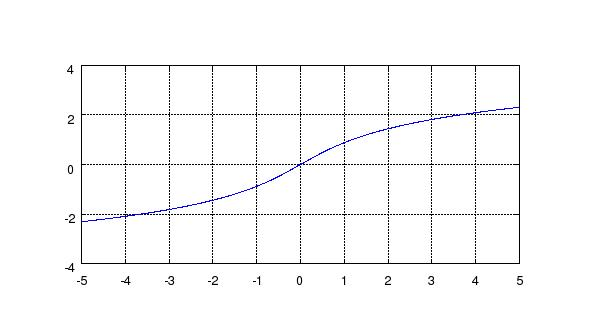
\includegraphics[width=8cm]{asinhplot}}

